
%% bare_jrnl.tex
%% V1.3
%% 2007/01/11
%% by Michael Shell
%% see http://www.michaelshell.org/
%% for current contact information.
%%
%% This is a skeleton file demonstrating the use of IEEEtran.cls
%% (requires IEEEtran.cls version 1.7 or later) with an IEEE journal paper.
%%
%% Support sites:
%% http://www.michaelshell.org/tex/ieeetran/
%% http://www.ctan.org/tex-archive/macros/latex/contrib/IEEEtran/
%% and
%% http://www.ieee.org/



% *** Authors should verify (and, if needed, correct) their LaTeX system  ***
% *** with the testflow diagnostic prior to trusting their LaTeX platform ***
% *** with production work. IEEE's font choices can trigger bugs that do  ***
% *** not appear when using other class files.                            ***
% The testflow support page is at:
% http://www.michaelshell.org/tex/testflow/


%%*************************************************************************
%% Legal Notice:
%% This code is offered as-is without any warranty either expressed or
%% implied; without even the implied warranty of MERCHANTABILITY or
%% FITNESS FOR A PARTICULAR PURPOSE! 
%% User assumes all risk.
%% In no event shall IEEE or any contributor to this code be liable for
%% any damages or losses, including, but not limited to, incidental,
%% consequential, or any other damages, resulting from the use or misuse
%% of any information contained here.
%%
%% All comments are the opinions of their respective authors and are not
%% necessarily endorsed by the IEEE.
%%
%% This work is distributed under the LaTeX Project Public License (LPPL)
%% ( http://www.latex-project.org/ ) version 1.3, and may be freely used,
%% distributed and modified. A copy of the LPPL, version 1.3, is included
%% in the base LaTeX documentation of all distributions of LaTeX released
%% 2003/12/01 or later.
%% Retain all contribution notices and credits.
%% ** Modified files should be clearly indicated as such, including  **
%% ** renaming them and changing author support contact information. **
%%
%% File list of work: IEEEtran.cls, IEEEtran_HOWTO.pdf, bare_adv.tex,
%%                    bare_conf.tex, bare_jrnl.tex, bare_jrnl_compsoc.tex
%%*************************************************************************

% Note that the a4paper option is mainly intended so that authors in
% countries using A4 can easily print to A4 and see how their papers will
% look in print - the typesetting of the document will not typically be
% affected with changes in paper size (but the bottom and side margins will).
% Use the testflow package mentioned above to verify correct handling of
% both paper sizes by the user's LaTeX system.
%
% Also note that the "draftcls" or "draftclsnofoot", not "draft", option
% should be used if it is desired that the figures are to be displayed in
% draft mode.
%
\documentclass[journal]{IEEEtran}
%
% If IEEEtran.cls has not been installed into the LaTeX system files,
% manually specify the path to it like:
% \documentclass[journal]{../sty/IEEEtran}





% Some very useful LaTeX packages include:
% (uncomment the ones you want to load)


% *** MISC UTILITY PACKAGES ***
%
%\usepackage{ifpdf}
% Heiko Oberdiek's ifpdf.sty is very useful if you need conditional
% compilation based on whether the output is pdf or dvi.
% usage:
% \ifpdf
%   % pdf code
% \else
%   % dvi code
% \fi
% The latest version of ifpdf.sty can be obtained from:
% http://www.ctan.org/tex-archive/macros/latex/contrib/oberdiek/
% Also, note that IEEEtran.cls V1.7 and later provides a builtin
% \ifCLASSINFOpdf conditional that works the same way.
% When switching from latex to pdflatex and vice-versa, the compiler may
% have to be run twice to clear warning/error messages.






% *** CITATION PACKAGES ***
%
%\usepackage{cite}
% cite.sty was written by Donald Arseneau
% V1.6 and later of IEEEtran pre-defines the format of the cite.sty package
% \cite{} output to follow that of IEEE. Loading the cite package will
% result in citation numbers being automatically sorted and properly
% "compressed/ranged". e.g., [1], [9], [2], [7], [5], [6] without using
% cite.sty will become [1], [2], [5]--[7], [9] using cite.sty. cite.sty's
% \cite will automatically add leading space, if needed. Use cite.sty's
% noadjust option (cite.sty V3.8 and later) if you want to turn this off.
% cite.sty is already installed on most LaTeX systems. Be sure and use
% version 4.0 (2003-05-27) and later if using hyperref.sty. cite.sty does
% not currently provide for hyperlinked citations.
% The latest version can be obtained at:
% http://www.ctan.org/tex-archive/macros/latex/contrib/cite/
% The documentation is contained in the cite.sty file itself.






% *** GRAPHICS RELATED PACKAGES ***
%
\ifCLASSINFOpdf
  % \usepackage[pdftex]{graphicx}
  % declare the path(s) where your graphic files are
  % \graphicspath{{../pdf/}{../jpeg/}}
  % and their extensions so you won't have to specify these with
  % every instance of \includegraphics
  % \DeclareGraphicsExtensions{.pdf,.jpeg,.png}
\else
  % or other class option (dvipsone, dvipdf, if not using dvips). graphicx
  % will default to the driver specified in the system graphics.cfg if no
  % driver is specified.
  % \usepackage[dvips]{graphicx}
  % declare the path(s) where your graphic files are
  % \graphicspath{{../eps/}}
  % and their extensions so you won't have to specify these with
  % every instance of \includegraphics
  % \DeclareGraphicsExtensions{.eps}
\fi
% graphicx was written by David Carlisle and Sebastian Rahtz. It is
% required if you want graphics, photos, etc. graphicx.sty is already
% installed on most LaTeX systems. The latest version and documentation can
% be obtained at: 
% http://www.ctan.org/tex-archive/macros/latex/required/graphics/
% Another good source of documentation is "Using Imported Graphics in
% LaTeX2e" by Keith Reckdahl which can be found as epslatex.ps or
% epslatex.pdf at: http://www.ctan.org/tex-archive/info/
%
% latex, and pdflatex in dvi mode, support graphics in encapsulated
% postscript (.eps) format. pdflatex in pdf mode supports graphics
% in .pdf, .jpeg, .png and .mps (metapost) formats. Users should ensure
% that all non-photo figures use a vector format (.eps, .pdf, .mps) and
% not a bitmapped formats (.jpeg, .png). IEEE frowns on bitmapped formats
% which can result in "jaggedy"/blurry rendering of lines and letters as
% well as large increases in file sizes.
%
% You can find documentation about the pdfTeX application at:
% http://www.tug.org/applications/pdftex





% *** MATH PACKAGES ***
%
%\usepackage[cmex10]{amsmath}
% A popular package from the American Mathematical Society that provides
% many useful and powerful commands for dealing with mathematics. If using
% it, be sure to load this package with the cmex10 option to ensure that
% only type 1 fonts will utilized at all point sizes. Without this option,
% it is possible that some math symbols, particularly those within
% footnotes, will be rendered in bitmap form which will result in a
% document that can not be IEEE Xplore compliant!
%
% Also, note that the amsmath package sets \interdisplaylinepenalty to 10000
% thus preventing page breaks from occurring within multiline equations. Use:
%\interdisplaylinepenalty=2500
% after loading amsmath to restore such page breaks as IEEEtran.cls normally
% does. amsmath.sty is already installed on most LaTeX systems. The latest
% version and documentation can be obtained at:
% http://www.ctan.org/tex-archive/macros/latex/required/amslatex/math/





% *** SPECIALIZED LIST PACKAGES ***
%
%\usepackage{algorithmic}
% algorithmic.sty was written by Peter Williams and Rogerio Brito.
% This package provides an algorithmic environment fo describing algorithms.
% You can use the algorithmic environment in-text or within a figure
% environment to provide for a floating algorithm. Do NOT use the algorithm
% floating environment provided by algorithm.sty (by the same authors) or
% algorithm2e.sty (by Christophe Fiorio) as IEEE does not use dedicated
% algorithm float types and packages that provide these will not provide
% correct IEEE style captions. The latest version and documentation of
% algorithmic.sty can be obtained at:
% http://www.ctan.org/tex-archive/macros/latex/contrib/algorithms/
% There is also a support site at:
% http://algorithms.berlios.de/index.html
% Also of interest may be the (relatively newer and more customizable)
% algorithmicx.sty package by Szasz Janos:
% http://www.ctan.org/tex-archive/macros/latex/contrib/algorithmicx/




% *** ALIGNMENT PACKAGES ***
%
%\usepackage{array}
% Frank Mittelbach's and David Carlisle's array.sty patches and improves
% the standard LaTeX2e array and tabular environments to provide better
% appearance and additional user controls. As the default LaTeX2e table
% generation code is lacking to the point of almost being broken with
% respect to the quality of the end results, all users are strongly
% advised to use an enhanced (at the very least that provided by array.sty)
% set of table tools. array.sty is already installed on most systems. The
% latest version and documentation can be obtained at:
% http://www.ctan.org/tex-archive/macros/latex/required/tools/


%\usepackage{mdwmath}
%\usepackage{mdwtab}
% Also highly recommended is Mark Wooding's extremely powerful MDW tools,
% especially mdwmath.sty and mdwtab.sty which are used to format equations
% and tables, respectively. The MDWtools set is already installed on most
% LaTeX systems. The lastest version and documentation is available at:
% http://www.ctan.org/tex-archive/macros/latex/contrib/mdwtools/


% IEEEtran contains the IEEEeqnarray family of commands that can be used to
% generate multiline equations as well as matrices, tables, etc., of high
% quality.


%\usepackage{eqparbox}
% Also of notable interest is Scott Pakin's eqparbox package for creating
% (automatically sized) equal width boxes - aka "natural width parboxes".
% Available at:
% http://www.ctan.org/tex-archive/macros/latex/contrib/eqparbox/





% *** SUBFIGURE PACKAGES ***
%\usepackage[tight,footnotesize]{subfigure}
% subfigure.sty was written by Steven Douglas Cochran. This package makes it
% easy to put subfigures in your figures. e.g., "Figure 1a and 1b". For IEEE
% work, it is a good idea to load it with the tight package option to reduce
% the amount of white space around the subfigures. subfigure.sty is already
% installed on most LaTeX systems. The latest version and documentation can
% be obtained at:
% http://www.ctan.org/tex-archive/obsolete/macros/latex/contrib/subfigure/
% subfigure.sty has been superceeded by subfig.sty.



%\usepackage[caption=false]{caption}
%\usepackage[font=footnotesize]{subfig}
% subfig.sty, also written by Steven Douglas Cochran, is the modern
% replacement for subfigure.sty. However, subfig.sty requires and
% automatically loads Axel Sommerfeldt's caption.sty which will override
% IEEEtran.cls handling of captions and this will result in nonIEEE style
% figure/table captions. To prevent this problem, be sure and preload
% caption.sty with its "caption=false" package option. This is will preserve
% IEEEtran.cls handing of captions. Version 1.3 (2005/06/28) and later 
% (recommended due to many improvements over 1.2) of subfig.sty supports
% the caption=false option directly:
%\usepackage[caption=false,font=footnotesize]{subfig}
%
% The latest version and documentation can be obtained at:
% http://www.ctan.org/tex-archive/macros/latex/contrib/subfig/
% The latest version and documentation of caption.sty can be obtained at:
% http://www.ctan.org/tex-archive/macros/latex/contrib/caption/

\usepackage{booktabs}
\usepackage{graphicx}
\usepackage{caption}
\usepackage{amsmath}

% *** FLOAT PACKAGES ***
%
%\usepackage{fixltx2e}
% fixltx2e, the successor to the earlier fix2col.sty, was written by
% Frank Mittelbach and David Carlisle. This package corrects a few problems
% in the LaTeX2e kernel, the most notable of which is that in current
% LaTeX2e releases, the ordering of single and double column floats is not
% guaranteed to be preserved. Thus, an unpatched LaTeX2e can allow a
% single column figure to be placed prior to an earlier double column
% figure. The latest version and documentation can be found at:
% http://www.ctan.org/tex-archive/macros/latex/base/



%\usepackage{stfloats}
% stfloats.sty was written by Sigitas Tolusis. This package gives LaTeX2e
% the ability to do double column floats at the bottom of the page as well
% as the top. (e.g., "\begin{figure*}[!b]" is not normally possible in
% LaTeX2e). It also provides a command:
%\fnbelowfloat
% to enable the placement of footnotes below bottom floats (the standard
% LaTeX2e kernel puts them above bottom floats). This is an invasive package
% which rewrites many portions of the LaTeX2e float routines. It may not work
% with other packages that modify the LaTeX2e float routines. The latest
% version and documentation can be obtained at:
% http://www.ctan.org/tex-archive/macros/latex/contrib/sttools/
% Documentation is contained in the stfloats.sty comments as well as in the
% presfull.pdf file. Do not use the stfloats baselinefloat ability as IEEE
% does not allow \baselineskip to stretch. Authors submitting work to the
% IEEE should note that IEEE rarely uses double column equations and
% that authors should try to avoid such use. Do not be tempted to use the
% cuted.sty or midfloat.sty packages (also by Sigitas Tolusis) as IEEE does
% not format its papers in such ways.


%\ifCLASSOPTIONcaptionsoff
%  \usepackage[nomarkers]{endfloat}
% \let\MYoriglatexcaption\caption
% \renewcommand{\caption}[2][\relax]{\MYoriglatexcaption[#2]{#2}}
%\fi
% endfloat.sty was written by James Darrell McCauley and Jeff Goldberg.
% This package may be useful when used in conjunction with IEEEtran.cls'
% captionsoff option. Some IEEE journals/societies require that submissions
% have lists of figures/tables at the end of the paper and that
% figures/tables without any captions are placed on a page by themselves at
% the end of the document. If needed, the draftcls IEEEtran class option or
% \CLASSINPUTbaselinestretch interface can be used to increase the line
% spacing as well. Be sure and use the nomarkers option of endfloat to
% prevent endfloat from "marking" where the figures would have been placed
% in the text. The two hack lines of code above are a slight modification of
% that suggested by in the endfloat docs (section 8.3.1) to ensure that
% the full captions always appear in the list of figures/tables - even if
% the user used the short optional argument of \caption[]{}.
% IEEE papers do not typically make use of \caption[]'s optional argument,
% so this should not be an issue. A similar trick can be used to disable
% captions of packages such as subfig.sty that lack options to turn off
% the subcaptions:
% For subfig.sty:
% \let\MYorigsubfloat\subfloat
% \renewcommand{\subfloat}[2][\relax]{\MYorigsubfloat[]{#2}}
% For subfigure.sty:
% \let\MYorigsubfigure\subfigure
% \renewcommand{\subfigure}[2][\relax]{\MYorigsubfigure[]{#2}}
% However, the above trick will not work if both optional arguments of
% the \subfloat/subfig command are used. Furthermore, there needs to be a
% description of each subfigure *somewhere* and endfloat does not add
% subfigure captions to its list of figures. Thus, the best approach is to
% avoid the use of subfigure captions (many IEEE journals avoid them anyway)
% and instead reference/explain all the subfigures within the main caption.
% The latest version of endfloat.sty and its documentation can obtained at:
% http://www.ctan.org/tex-archive/macros/latex/contrib/endfloat/
%
% The IEEEtran \ifCLASSOPTIONcaptionsoff conditional can also be used
% later in the document, say, to conditionally put the References on a 
% page by themselves.





% *** PDF, URL AND HYPERLINK PACKAGES ***
%
%\usepackage{url}
% url.sty was written by Donald Arseneau. It provides better support for
% handling and breaking URLs. url.sty is already installed on most LaTeX
% systems. The latest version can be obtained at:
% http://www.ctan.org/tex-archive/macros/latex/contrib/misc/
% Read the url.sty source comments for usage information. Basically,
% \url{my_url_here}.





% *** Do not adjust lengths that control margins, column widths, etc. ***
% *** Do not use packages that alter fonts (such as pslatex).         ***
% There should be no need to do such things with IEEEtran.cls V1.6 and later.
% (Unless specifically asked to do so by the journal or conference you plan
% to submit to, of course. )


% correct bad hyphenation here
\hyphenation{op-tical net-works semi-conduc-tor}

%\onecolumn
\begin{document}
%
% paper title
% can use linebreaks \\ within to get better formatting as desired
\title{Analysis of Genetic Programming Techniques for Unbalanced Data}
%
%
% author names and IEEE memberships
% note positions of commas and nonbreaking spaces ( ~ ) LaTeX will not break
% a structure at a ~ so this keeps an author's name from being broken across
% two lines.
% use \thanks{} to gain access to the first footnote area
% a separate \thanks must be used for each paragraph as LaTeX2e's \thanks
% was not built to handle multiple paragraphs
%

\author{Jessica Pauli de C. Bonson, Dalhousie University}

% note the % following the last \IEEEmembership and also \thanks - 
% these prevent an unwanted space from occurring between the last author name
% and the end of the author line. i.e., if you had this:
% 
% \author{....lastname \thanks{...} \thanks{...} }
%                     ^------------^------------^----Do not want these spaces!
%
% a space would be appended to the last name and could cause every name on that
% line to be shifted left slightly. This is one of those "LaTeX things". For
% instance, "\textbf{A} \textbf{B}" will typeset as "A B" not "AB". To get
% "AB" then you have to do: "\textbf{A}\textbf{B}"
% \thanks is no different in this regard, so shield the last } of each \thanks
% that ends a line with a % and do not let a space in before the next \thanks.
% Spaces after \IEEEmembership other than the last one are OK (and needed) as
% you are supposed to have spaces between the names. For what it is worth,
% this is a minor point as most people would not even notice if the said evil
% space somehow managed to creep in.



% If you want to put a publisher's ID mark on the page you can do it like
% this:
%\IEEEpubid{0000--0000/00\$00.00~\copyright~2007 IEEE}
% Remember, if you use this you must call \IEEEpubidadjcol in the second
% column for its text to clear the IEEEpubid mark.



% use for special paper notices
%\IEEEspecialpapernotice{(Invited Paper)}




% make the title area
\maketitle


\begin{abstract}
%\boldmath
In this work Genetic Programming techniques are explored to improve the performance on unbalanced datasets. The initial system uses linear GP,  modularity, sampling heuristics and dynamic structures. The methods analyzed are introns removal, complex instruction set, and diversity maintenance mechanisms. The results were compared using statistical methods, and were proved to improve the system performance, complexity, and runtime.
\end{abstract}
% IEEEtran.cls defaults to using nonbold math in the Abstract.
% This preserves the distinction between vectors and scalars. However,
% if the journal you are submitting to favors bold math in the abstract,
% then you can use LaTeX's standard command \boldmath at the very start
% of the abstract to achieve this. Many IEEE journals frown on math
% in the abstract anyway.

% Note that keywords are not normally used for peerreview papers.
\begin{IEEEkeywords}
machine learning, linear genetic programming, diversity maintenance
\end{IEEEkeywords}






% For peer review papers, you can put extra information on the cover
% page as needed:
% \ifCLASSOPTIONpeerreview
% \begin{center} \bfseries EDICS Category: 3-BBND \end{center}
% \fi
%
% For peerreview papers, this IEEEtran command inserts a page break and
% creates the second title. It will be ignored for other modes.
\IEEEpeerreviewmaketitle



\section{Introduction}
% The very first letter is a 2 line initial drop letter followed
% by the rest of the first word in caps.
% 
% form to use if the first word consists of a single letter:
% \IEEEPARstart{A}{demo} file is ....
% 
% form to use if you need the single drop letter followed by
% normal text (unknown if ever used by IEEE):
% \IEEEPARstart{A}{}demo file is ....
% 
% Some journals put the first two words in caps:
% \IEEEPARstart{T}{his demo} file is ....
% 
% Here we have the typical use of a "T" for an initial drop letter
% and "HIS" in caps to complete the first word.
\IEEEPARstart{T}{his} project expands the previous work on the class sandboxes to test and understand additional features for Genetic Programming (GP). The goal is to find which new features are capable of improving the performance of the system on unbalanced datasets. The modified system will be benchmarked against the results of the current system for the datasets Thyroid \cite{thyroid} and Shuttle \cite{shuttle}, focusing on the later. This works assumes that all classes are equally important, so the benchmark is based on the class-wise detection rate (DR) metric. The methods tested in this work are introns removal, non-linear instructions, and diversity maintenance approaches.
The next paper sections are organized as follows. Section 2 explains the current system implementation and present the benchmark. Section 3 analyzes an initial tuning on the parameters and restrictions on the runs. In Section 4 results regarding introns removal and complex instruction set are presented. Section 5 explore three diversity maintenance approaches. The final results for the datasets are shown on Section 6. Finally, Section 7 presents the conclusion and future work.

\section{System Implementation and Benchmark}
The system currently implemented is a GP algorithm for multi-class classification using linear representation. The system is able to evolve modular behaviors using teams of programs. Each program has an action, where an action means the class that the program will output a membership value. In a team, the program with the highest output value defines what class the team will classify the input. At each generation, a percentage of worst teams are replaced. If a program no longer participates in any team because of them were removed, then it is also removed. The system replaces the removed programs by cloning the same number of programs from the resulting population using uniform probability. There are three types of mutations for programs. The first  mutation randomly selects an instruction and make a small change, e.g. using another registers as the target or using another arithmetic operation. The second and third mutations randomly add and remove an instruction. After creating the new programs, new teams are produced by cloning the remaining teams using proportional selection based on their fitness. Two mutations may affect a clone, adding or removing a program. If a program is added, it must be one of the newly created programs.

Other relevant features of the current system are: both the team size and the instruction size of the programs are variable, so the solutions structure are dynamic; a balanced sampling heuristic with oversampling is used to obtain the training data each generation, in order to ensure the solutions learn the patterns for all classes; the stop criterion is simply the end of the last generation; and the fitness function is the accuracy metric. The parameters used to run the system for the Thyroid and Shuttle datasets are shown in Table \ref{table:initial_config}. The parameters were chosen so that they would give a good performance in a suitable time. Due to different amount of classes to be learned, each dataset uses a different maximum of programs per team. For this configuration, the best solution across 30 runs is 0.94 for the Thyroid dataset and 0.425 for the Shuttle dataset. 

\begin{table}[h]
\centering
\captionsetup{justification=centering}
\begin{tabular}{@{}ll@{}}
\toprule
Programs Population & 400 \\
Teams Population    & 200 \\
Total Generations   & 20  \\
Total Runs          & 30 \\
Total Registers          & 2 (1 output and 1 extra) \\
Team Replacement Rate          & 0.2 \\
Point Replacement Rate          & 1.0 \\
Sampling Size          & 120 \\
\midrule
Change Instruction Mutation          & 0.9 \\
Add Instruction Mutation          & 0.9 \\
Remove Instruction Mutation          & 0.8 \\
Add Program Mutation          & 0.8 \\
Remove Program Mutation          & 0.7 \\
\midrule
Min. Program Size          & 	1 \\
Max. Program Size          & 30 \\
Initial Program Size          & 10 \\
\midrule
Min. Team Size          &  2 \\
Max. Team Size          & 9 (Thyroid), 14 (Shuttle) \\
Initial Team Size          & 3 \\
\bottomrule
\end{tabular}
\caption{Initial system configuration.}
\label{table:initial_config}
\end{table}

\section{Parameters Tuning}
Initially this work attempted to use the parameters from the previous section as the baseline to apply the new GP techniques. However, the system performed very poorly, and mainly due to the small number of generations the diversity maintenance methods ended up producing worse results than the benchmark. So various modifications were made from the previous runs to attempt to improve the results. The initial implementation replaced all data points at each generation, this was modified to a replacement rate of 0.2, in order to modify the environment smoothly so the solutions would be able to continuously adapt to it. The team replacement rate was modified to 0.6, so it would evolve faster than the environment. The populations were modified from 400 programs and 200 teams to 160 programs and 80 teams, and the generations from 20 to 500. This modification intend to give the solutions more time to evolve and benefit from diversity maintenance techniques. Restrictions were also added, they ensure that all teams always have at least one action per class. Since the final objective is to obtain a detection rate of 100% for all classes, it seems natural to enforce this rule as a transfer of knowledge. The last modification was to add mutation rate of actions, in order to avoid the dominance of an action over the others in the population.

The most relevant change was the modification of the generations and populations. The new best solutions are 0.97 and 0.74, respectively. The results improved with significance at p less than or equal to 0.01, using the Mann-Whitney U-Test. The modification of the point replacement rate, the balance restrictions, and the action mutation didn't significantly improved the results, but were maintained in order to ensure the best functionality of the algorithm. The final choice of parameters is shown on Table \ref{table:improved_config}.

\begin{table}[h]
\centering
\captionsetup{justification=centering}
\begin{tabular}{@{}ll@{}}
\toprule
Programs Population & 160 \\
Teams Population    & 80 \\
Total Generations   & 500 \\
Total Runs          & 30 \\
Total Registers          & 2 (1 output and 1 extra) \\
Team Replacement Rate          & 0.6 \\
Point Replacement Rate          & 0.2 \\
Sampling Size          & 120 \\
\midrule
Change Instruction Mutation          & 0.9 \\
Change Action Mutation          & 0.1 \\
Add Instruction Mutation          & 0.9 \\
Remove Instruction Mutation          & 0.8 \\
Add Program Mutation          & 0.8 \\
Remove Program Mutation          & 0.7 \\
\midrule
Min. Program Size          & 	1 \\
Max. Program Size          & 30 \\
Initial Program Size          & 10 \\
\midrule
Min. Team Size          &  total classes \\
Max. Team Size          & 9 (Thyroid), 14 (Shuttle) \\
Initial Team Size          & total classes \\
\bottomrule
\end{tabular}
\caption{Improved system configuration.}
\label{table:improved_config}
\end{table}

\section{Non-Linear Instructions and Introns Removal}
The first feature added to the system is non-linear instructions: ln, exp, cos, if <, and if >=. To work around the problem of overflow, if an overflow occurs the returned result is the variable value before the execution of the operation. The hypothesis is that non-linear instructions will result in a higher accuracy, that leads to a higher DR.  A better accuracy is expected since now problems will be able to increase their complexity to match complex data patterns. The second experiment is to add introns removal to the GP algorithm, so instructions with no effect on the final output are ignored while processing the instruction set. It is expected that the runtime performance will improve, without affecting the DR performance.

The results for the combination of runs using the simple and complex set instructions, with and without introns removal for 10 runs is shown on Table \ref{table:runtime}. For both cases the introns removal successfully reduced the runtime for both sets of instructions. The main difference occurs in the complex set, where the introns removal was able to reduce the runtime by almost half of the total time. Since the complex set includes the instruction 'if', that when it is detected to be an intron it is fully removed along with its instruction and the following 'if' instructions, introns removal affect the complex instructions set to a greater extent.

The analysis of the DR performance showed that for both datasets there are statistically no difference between using the simple or the complex set of instructions. This may have occurred because these datasets don't get a great benefit out of complexity. However, the interesting result is that using the complex instruction set and introns removal the system was able to maintain the same performance running on nearly half the time.

\begin{table}[h]
\centering
\captionsetup{justification=centering}
\begin{tabular}{@{}lll@{}}
\toprule
Thyroid Dataset &  Avg. Runtime &  Std. Dev. Runtime\\
\midrule
Linear Instructions    & 985  & 88 \\
Linear Instructions + Introns Removal   & 827  & 89 \\
Complex Instructions    & 1016  & 271 \\
Complex Instructions + Introns Removal   & 596  & 92 \\
\midrule
Shuttle Dataset & Avg. Runtime &  Std. Dev. Runtime \\
\midrule
Linear Instructions    & 3703  & 396 \\
Linear Instructions + Introns Removal   & 3270  & 495 \\
Complex Instructions    & 3741  & 122 \\
Complex Instructions + Introns Removal   & 2083  & 303 \\
\bottomrule
\end{tabular}
\caption{Runtimes in seconds for intron removal and instructions sets.}
\label{table:runtime}
\end{table}

\section{Diversity Maintenance Methods}
In this section analyzes how genotypic and behavioural diversity maintenance affects the system performance. The genotypic distance will be calculated using the method described by \cite{ref3}, where the distance between teams is the the ratio of active programs common to both teams. An active program is one that was selected at least once by the team to produce the output of the team. The diversity is calculated as the average of the pairwise distance between the K-Nearest Neighbors (KNN) across the genotype distance search space, with k = 8. The objective of using KNN in this context is to give a higher fitness to individuals that occupy a sparse local region in genotypic space. The fitness is calculated by the formula (1-p)*(raw fitness) + p*diversity, where p can be tuned to modify the weight of the parameters. The p value used is 0.1, selected empirically.

The behavioral diversity will be calculated using fitness sharing as defined in \cite{ref4}, where individuals share their fitness on the correct classified a samples. Therefore individuals are rewarded by performing well against specific samples that other individuals are not able to classify. A second behavioral diversity maintenance method is a modified version of fitness sharing, named class-wise fitness sharing. The formula is modified so the fitness sharing is calculated separately for each class, and then averaged by the total number of classes. The goal of this modified version is to ensure that fitness sharing it prioritizing classes with more samples.

All the comparisons were performed using the Mann-Whitney U-Test for 30 runs and for p less than or equal to 0.05. For the Thyroid dataset, there was no statistically significant improvement across the diversity maintenance methods. I attempted to obtain better results by doubling the total of generations and increasing the number of runs, but the results still had no significant differences. For the Shuttle dataset both fitness sharing methods were outperformed by the default configuration, with no diversity maintenance. Also, there was no significant difference between the class-wise and traditional fitness sharing. For both the training fitness of the solutions varied around 0.01, the best one was only 0.024. It seems that the fitness sharing enforced a policy where it was nearly impossible to get a good fitness and it improved at very small steps, so the search in the landscape wasn't able to evolve. Although the bad results for fitness sharing, for the Shuttle dataset the genotype diversity maintenance method was able to perform similarly to the default configuration and produced the final best solution. It is worth noting that the genotype diversity method with complex instructions was able to outperform the one with simple instructions. So besides the previous results of statistically irrelevant differences between the simple and complex instructions set, and between the no diversity maintenance and genotype diversity maintenance, the combination of the complex set with genotype diversity actually produced an improvement in the class-wise detection rate.

Figure \ref{fig:recalls} compares de class-wise detection rate over the generations for each class for the four methods. It is clear that the fitness sharing method was not being able to stabilize over generations, probably due to problems pointed in the behavior of the fitness values. The class-wise fitness sharing plot is now being shown since it also had this problem.  Regarding the default method and the genotype diversity maintenance method, the charts show that the diversity maintenance method was able to improve the population evolution so that the classes are learned more smoothly and continuosly over time.

\begin{figure}[!t]
  \centering
  \captionsetup{justification=centering}
  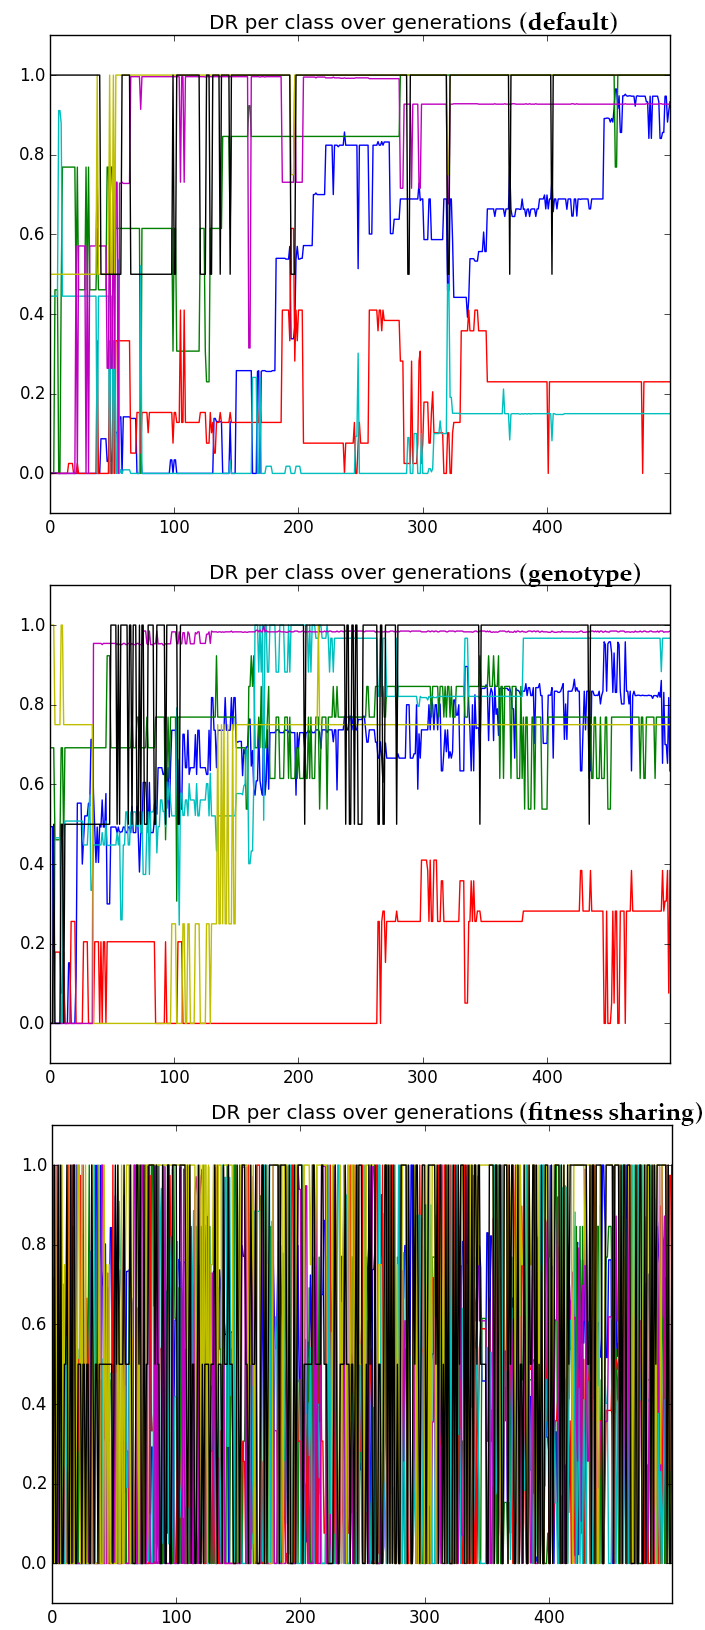
\includegraphics[width=3.0in]{images/recalls}
  \caption{Comparison of DR per class over generations.}
  \label{fig:recalls}
\end{figure}

\section{Final Result}
The previous sections focused on improving the distribution of the results, this section will analyze how these improvements affected the final solution. Since the most significant differences were shown on the Shuttle dataset, that is also the more complex dataset, this will be the focus of this section. The initial best result for the Shuttle dataset was a DR of 0.42563, with a recall of 0.71, 0.54, 0.0, 0.0, 0.73, 0.0, 1.0, respectively for the classes 0 to 6. The final solution had four programs, with actions for the classes 0, 1, 4, and 6, the only ones were it was able to get a good recall. The average runtime was 82 seconds, and each program had around 10.75 instructions. After the modifications on Section 3, the system was improved and the best solution got a DR of 0.74, with recalls 0.83, 0.77, 0.33, 0.33, 0.92, 1.0, 1.0. The best team had 14 programs, with at least one for each class, four programs for class 0, two for classes 1, 2, 5 and 6. Each program had an average of 11.64 overall instruction, with around 10.21 non-intron instructions. The mean runtime was 3300 seconds. Adding the complex instructions set and intron removal on Section 4 gave an equivalent final solution performance, but composed of only 11 programs, with a decreased mean runtime (2129 seconds), 12.36 overall instructions, and 6.54 effective instructions per program. So adding the complex instruction set reduced the overall complexity of the final team without reducing its performance. Finally, by adding the genotype diversity maintenance on Section 5, the final solution was able to obtain a DR equal to 0.784 with the cost of the runtime increasing just by 0.03. The recall per class was 0.63, 0.77, 0.38, 0.97, 0.98, 0.75, 1.0. The total programs in the final team was also 11, but now no class had more than 2 programs dedicated to it, so the recalls per class were more balanced. There was no significative difference regarding the total of instructions.

\section{Conclusion}
This paper presented an investigatory analysis of GP techniques on the unbalanced datasets Thyroid and Shuttle. The methods studied were intron removal, complex instructions sets and the following diversity maintenance approaches: fitness sharing, classwise fitness sharing, and genotype diversity based on active programs in the teams. As expected, introns removal decreased the runtime of the algorithm, mainly when coupled with the complex instruction set. The fitness sharing methods didn't provide significant improvements, and it would be necessary to further study them in this domain to understand why they are not improving the algorithm performance. The genotype diversity maintenance along with the complex instructions set and introns removal sucessfully improved the solutions while decreasing their complexity and runtime. An initial work on the balance between the genotype diversity and the fitness showed to significant differences across balance values between 0.1 and 0.3, but it would be interesting to try to find the better balance between them in order to obtain the best performance improvement. Other future works would be investigate how pareto and multi-objetive methods would interact with GP for these unbalanced datasets.

% An example of a floating figure using the graphicx package.
% Note that \label must occur AFTER (or within) \caption.
% For figures, \caption should occur after the \includegraphics.
% Note that IEEEtran v1.7 and later has special internal code that
% is designed to preserve the operation of \label within \caption
% even when the captionsoff option is in effect. However, because
% of issues like this, it may be the safest practice to put all your
% \label just after \caption rather than within \caption{}.
%
% Reminder: the "draftcls" or "draftclsnofoot", not "draft", class
% option should be used if it is desired that the figures are to be
% displayed while in draft mode.
%
%\begin{figure}[!t]
%\centering
%\includegraphics[width=2.5in]{myfigure}
% where an .eps filename suffix will be assumed under latex, 
% and a .pdf suffix will be assumed for pdflatex; or what has been declared
% via \DeclareGraphicsExtensions.
%\caption{Simulation Results}
%\label{fig_sim}
%\end{figure}

% Note that IEEE typically puts floats only at the top, even when this
% results in a large percentage of a column being occupied by floats.


% An example of a double column floating figure using two subfigures.
% (The subfig.sty package must be loaded for this to work.)
% The subfigure \label commands are set within each subfloat command, the
% \label for the overall figure must come after \caption.
% \hfil must be used as a separator to get equal spacing.
% The subfigure.sty package works much the same way, except \subfigure is
% used instead of \subfloat.
%
%\begin{figure*}[!t]
%\centerline{\subfloat[Case I]\includegraphics[width=2.5in]{subfigcase1}%
%\label{fig_first_case}}
%\hfil
%\subfloat[Case II]{\includegraphics[width=2.5in]{subfigcase2}%
%\label{fig_second_case}}}
%\caption{Simulation results}
%\label{fig_sim}
%\end{figure*}
%
% Note that often IEEE papers with subfigures do not employ subfigure
% captions (using the optional argument to \subfloat), but instead will
% reference/describe all of them (a), (b), etc., within the main caption.


% An example of a floating table. Note that, for IEEE style tables, the 
% \caption command should come BEFORE the table. Table text will default to
% \footnotesize as IEEE normally uses this smaller font for tables.
% The \label must come after \caption as always.
%
%\begin{table}[!t]
%% increase table row spacing, adjust to taste
%\renewcommand{\arraystretch}{1.3}
% if using array.sty, it might be a good idea to tweak the value of
% \extrarowheight as needed to properly center the text within the cells
%\caption{An Example of a Table}
%\label{table_example}
%\centering
%% Some packages, such as MDW tools, offer better commands for making tables
%% than the plain LaTeX2e tabular which is used here.
%\begin{tabular}{|c||c|}
%\hline
%One & Two\\
%\hline
%Three & Four\\
%\hline
%\end{tabular}
%\end{table}


% Note that IEEE does not put floats in the very first column - or typically
% anywhere on the first page for that matter. Also, in-text middle ("here")
% positioning is not used. Most IEEE journals use top floats exclusively.
% Note that, LaTeX2e, unlike IEEE journals, places footnotes above bottom
% floats. This can be corrected via the \fnbelowfloat command of the
% stfloats package.


% Can use something like this to put references on a page
% by themselves when using endfloat and the captionsoff option.
\ifCLASSOPTIONcaptionsoff
  \newpage
\fi



% trigger a \newpage just before the given reference
% number - used to balance the columns on the last page
% adjust value as needed - may need to be readjusted if
% the document is modified later
%\IEEEtriggeratref{8}
% The "triggered" command can be changed if desired:
%\IEEEtriggercmd{\enlargethispage{-5in}}

% references section

% can use a bibliography generated by BibTeX as a .bbl file
% BibTeX documentation can be easily obtained at:
% http://www.ctan.org/tex-archive/biblio/bibtex/contrib/doc/
% The IEEEtran BibTeX style support page is at:
% http://www.michaelshell.org/tex/ieeetran/bibtex/
%\bibliographystyle{IEEEtran}
% argument is your BibTeX string definitions and bibliography database(s)
%\bibliography{IEEEabrv,../bib/paper}
%
% <OR> manually copy in the resultant .bbl file
% set second argument of \begin to the number of references
% (used to reserve space for the reference number labels box)
\bibliographystyle{IEEEtran}
\bibliography{example}

% that's all folks
\end{document}


